% arara: xelatex: { synctex: yes, shell: yes }
\documentclass[convert={density=300,size=1500x1500,outext=.png}]{standalone}

\usepackage{fontspec}
\setmainfont[Ligatures={Required,Common,Contextual,Rare,Historic,TeX},Numbers=OldStyle,RawFeature={+ss05,+dlig,+hlig,+calt,+liga},ItalicFeatures={RawFeature={+cv04,+clig,+swsh,+calt,+liga,+hlig,+ss05},CharacterVariant=5:0}]{EB Garamond}
\usepackage{eulervm}

\usepackage{graphicx}
\usepackage{xcolor}

\usepackage{tikz}
\usetikzlibrary{patterns}

%\definecolor{ct}{rgb}{1,0,0}
%\definecolor{pf}{rgb}{1,0,0}
\definecolor{bg}{RGB}{253,246,227}

\begin{document}

\pagecolor{bg}

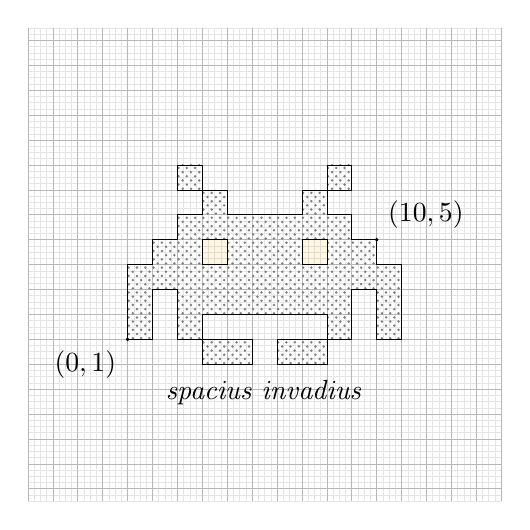
\begin{tikzpicture}[x=9pt,y=9pt]
	\tikzstyle{ct} = [draw,very thin,color=black];
	\tikzstyle{pf} = [fill,pattern=crosshatch dots,pattern color=gray];
	\draw [step=0.25,draw,very thin,opacity=0.1] (-4,-5.5) grid (15,13.5);
	\draw [step=1,draw,very thin,opacity=0.2] (-4,-5.5) grid (15,13.5);
	\path [pf] (0,1) -- (0,4) -- (1,4) -- (1,5) -- (2,5) -- (2,6) -- (3,6) -- (3,7) -- (4,7) -- (4,6) -- (7,6) -- (7,7) -- (8,7) -- (8,6) -- (9,6) -- (9,5) -- (10,5) -- (10,4) -- (11,4) -- (11,1) -- (10,1) -- (10,3) -- (9,3) -- (9,1) -- (8,1) -- (8,2) -- (3,2) -- (3,1) -- (2,1) -- (2,3) -- (1,3) -- (1,1) -- cycle;
	\path [pf] (3,7) -- (2,7) -- (2,8) -- (3,8) -- cycle;
	\path [pf] (8,7) -- (8,8) -- (9,8) -- (9,7) -- cycle;
	\path [pf] (3,1) -- (5,1) -- (5,0) -- (3,0) -- cycle;
	\path [pf] (8,1) -- (6,1) -- (6,0) -- (8,0) -- cycle;
	\path [fill=bg] (3,4) -- (3,5) -- (4,5) -- (4,4) -- cycle;
	\path [fill=bg] (7,4) -- (7,5) -- (8,5) -- (8,4) -- cycle;
	\draw [step=0.25,draw,very thin,opacity=0.1] (3,4) grid (4,5);
	\draw [step=0.25,draw,very thin,opacity=0.1] (7,4) grid (8,5);
	\path [ct] (0,1) -- (0,4) -- (1,4) -- (1,5) -- (2,5) -- (2,6) -- (3,6) -- (3,7) -- (4,7) -- (4,6) -- (7,6) -- (7,7) -- (8,7) -- (8,6) -- (9,6) -- (9,5) -- (10,5) -- (10,4) -- (11,4) -- (11,1) -- (10,1) -- (10,3) -- (9,3) -- (9,1) -- (8,1) -- (8,2) -- (3,2) -- (3,1) -- (2,1) -- (2,3) -- (1,3) -- (1,1) -- cycle;
	\path [ct] (3,7) -- (2,7) -- (2,8) -- (3,8) -- cycle;
	\path [ct] (8,7) -- (8,8) -- (9,8) -- (9,7) -- cycle;
	\path [ct] (3,1) -- (5,1) -- (5,0) -- (3,0) -- cycle;
	\path [ct] (8,1) -- (6,1) -- (6,0) -- (8,0) -- cycle;
	\path [ct] (3,4) -- (3,5) -- (4,5) -- (4,4) -- cycle;
	\path [ct] (7,4) -- (7,5) -- (8,5) -- (8,4) -- cycle;
	\node at (0,1) [circle,fill=black,inner sep=0.5pt,label={-135:$(0,1)$}] {};
	\node at (10,5) [circle,fill=black,inner sep=0.5pt,label={45:$(10,5)$}] {};
	\node at (5.5,-0.25) [anchor=north,align=center] {\textit{spacius invadius}};
\end{tikzpicture}

\end{document}
